\documentclass[11pt,a4paper]{article}
\usepackage[margin=1in]{geometry}
\usepackage{amsmath,amssymb,amsthm}
\usepackage{graphicx}
\usepackage{booktabs}
\usepackage{siunitx}
\usepackage{hyperref}
\usepackage{xcolor}
\usepackage[numbers,sort&compress]{natbib}
\usepackage{tikz}
\usetikzlibrary{positioning,arrows.meta}
\usepackage{pgfplots}
\pgfplotsset{compat=1.18}
\usepackage{caption}
\usepackage{listings}
\usepackage{array}
\captionsetup{font=small,labelfont=bf}
\hypersetup{colorlinks=true,linkcolor=blue!50!black,citecolor=blue!50!black,urlcolor=blue!50!black}

% text colour tier badges (font-independent; NO emoji)
\newcommand{\tierbadge}[2]{\textcolor{#1}{\textbf{[#2]}}}
\providecommand{\tierBlue}{\tierbadge{blue!60!black}{BLUE}}
\providecommand{\tierGreen}{\tierbadge{green!45!black}{GREEN}}
\providecommand{\tierYellow}{\tierbadge{yellow!50!black}{CITE}}
\providecommand{\tierOrange}{\tierbadge{orange!80!black}{ORANGE}}
\providecommand{\tierRed}{\tierbadge{red!75!black}{RED}}

\title{
  \textbf{An in-silico senolytic-enabled regimen for osteoarthritic
  cartilage regeneration}\\[4pt]
  \large A structural result: osteoarthritis is the hardest of the four
  senolytic-closable degenerative cures, and niche senescent-cell clearance
  is the key that closes its $\geq 90\%$ restoration gate
}
\author{
  \texttt{demiurge} maintainers\\
  \normalsize\textit{dancinlab}\\[2pt]
  \normalsize\href{https://github.com/dancinlab/demiurge}{\texttt{github.com/dancinlab/demiurge}}
}
\date{\today}
\begin{document}
\maketitle

\begin{abstract}
We report an in-silico structural analysis of osteoarthritic (OA) cartilage as a
complete-restoration cure target, as one instance of the universal
neogenesis-bottleneck framework. We decompose the diseased joint surface into three
cell-state classes by their distance from recoverability --- reversible chondrocytes
(mass $0.35$, achievable efficiency $\eta=0.90$), dormant progenitors ($0.30$,
$\eta=0.75$), and fibrillated/lost cartilage ($0.35$, $\eta_{\text{lost}}=0.40$) --- and
drive each to its best-achievable efficiency under a pre-registered $\geq 90\%$-of-normal
restoration gate. Reactivation and reversal of the surviving classes saturate the cure
ceiling at $0.68$, \emph{below} the gate, which therefore \textbf{BLOCKS}; the unmet
residual is the same single binding axis the framework predicts: neogenesis of the lost
class --- here, chondral neogenesis. The lost-class efficiency $\eta_{\text{lost}}=0.40$
is the \emph{lowest} among the four senolytic-closable cures, making OA the hardest of
them. We then show that clearance of regenerative-niche senescent cells lifts the lost
(and partly the dormant) efficiency, $\eta_{\text{lost}}(\phi)=0.40+0.60\,\phi$, and that
the restoration ceiling crosses the gate at a senescent-clearance fraction
$\phi^\ast\!\approx\!78\%$. The regeneration arm pairs chondral neogenesis with
load-bearing matrix maturation. A domain-specific constraint is that cartilage is
\emph{avascular}: intra-articular delivery is the secondary binding axis. The senolytic
leg is motivated by an established finding --- senescent chondrocytes drive OA matrix
degradation and are a validated senolytic target. The contribution is structural and
deterministic within the manifest assumptions; we claim no efficacy, the efficiencies
are literature-order (flagged \tierOrange), and the ordering that produces the
bottleneck is robust to their exact values (\tierGreen). Reproduction artifacts:
\texttt{exports/OA-CURE/}.
\end{abstract}

\section{Introduction}
\label{sec:intro}
A disease-modifying cure for osteoarthritis --- not symptom control (analgesia,
viscosupplementation) but restoration of a hyaline joint surface toward a
never-diseased state --- has no approved instance. OA is the most prevalent joint
disease and a leading cause of disability worldwide \citep{hunter2019}; articular
cartilage, once fibrillated, does not spontaneously regenerate, because it is avascular,
aneural, and sparsely cellular, with chondrocytes embedded in a slow-turnover matrix
\citep{sophia2009}. Existing restorative techniques --- microfracture, autologous
chondrocyte implantation \citep{brittberg1994}, osteochondral grafting, tissue-engineered
scaffolds \citep{makris2015} --- repair focal defects with predominantly fibrocartilage,
not durable load-bearing hyaline tissue, and do not arrest the global degenerative
process.

We analyse OA not in isolation but as one \emph{instance} of a general framework
(the universal neogenesis-bottleneck). The framework decomposes any chronic-degenerative
field into three cell-state classes by recoverability --- surviving-but-impaired cells
that respond to reversal (\emph{reversible}), quiescent stem/progenitors that respond to
reactivation (\emph{dormant}), and tissue that is gone, whose niche must be rebuilt
(\emph{lost/fibrosed}) --- and asks which class is the binding constraint on a cure. The
decomposition is deliberately coarse (three numbers): the claim under test is not
quantitative efficacy but \emph{which class binds}, a question robust to coarse inputs.
For OA the answer is unambiguous and, within the framework, the most extreme: the lost
fibrillated-cartilage class has the lowest achievable efficiency of any of the four
senolytic-closable cures, so OA is the hardest of them, and chondral neogenesis is the
single residual axis.

\medskip\noindent\textbf{Contributions.}
\begin{enumerate}\itemsep0.3em
\item \textbf{OA as the hardest senolytic-closable cure.} The OA manifest blocks the
$\geq 90\%$ gate at a best-achievable ceiling of $0.68$, on the binding axis
$\eta_{\text{lost}}=0.40$ --- the lowest lost-class efficiency among the four cures
(Fig.~\ref{fig:classdecomp}, Tab.~\ref{tab:manifest}).
\item \textbf{A senolytic key.} Niche senescent-cell clearance lifts the lost-class
efficiency; the restoration ceiling crosses the gate at clearance
$\phi^\ast\!\approx\!78\%$ (Fig.~\ref{fig:senolytic}).
\item \textbf{An honest, avascular-aware regimen.} The regeneration arm is chondral
neogenesis $+$ load-bearing matrix maturation; the secondary binding axis is
intra-articular delivery into avascular cartilage.
\end{enumerate}

\section{Background}
\label{sec:bg}
\paragraph{Articular cartilage and why it does not heal.} Hyaline articular cartilage is
an avascular, aneural, lymphatic-free connective tissue: chondrocytes occupy only
${\sim}1$--$5\%$ of its volume and are nourished by diffusion through the synovial fluid
and subchondral plate \citep{sophia2009}. This architecture --- which gives cartilage its
low-friction, load-bearing competence --- is also why it cannot mount a vascular wound
response: there is no blood supply to deliver progenitors, cytokines, or systemic drug.
Consequently, lost matrix is replaced (if at all) by mechanically inferior fibrocartilage
\citep{makris2015}. The avascularity is therefore simultaneously the source of the
disease's intractability and the chief delivery constraint on any therapy.

\paragraph{Cell-state gradient in the osteoarthritic joint.} The OA surface presents the
same recoverability gradient the framework assumes. Some chondrocytes are
surviving-but-dysfunctional, shifting toward a catabolic, hypertrophic, or
senescence-associated secretory (SASP) phenotype but in principle reversible; a dormant
progenitor reservoir exists (marrow-derived and synovium/surface progenitors) and is
chondrogenic when reactivated \citep{johnstone1998}; and a fraction of the surface is
frankly fibrillated/eroded --- the lost class whose hyaline structure must be rebuilt de
novo \citep{loeser2016}.

\paragraph{Senescent chondrocytes drive OA --- the senolytic rationale.} Cellular
senescence is now established as a driver of OA pathogenesis, not a bystander: senescent
chondrocytes accumulate in OA cartilage and sustain a SASP that degrades matrix and
propagates dysfunction to neighbouring cells \citep{coryell2021,loeser2016}. Critically,
\emph{local} clearance of senescent cells in a post-traumatic OA model attenuated disease
and created a pro-regenerative environment \citep{jeon2017}, and systemic senolytics
improve physical function in aged animals \citep{xu2018}. Senescent cells are thus a
\emph{validated} therapeutic target in OA, and the senescent niche is a paracrine brake
on the resident progenitor pool --- exactly the upstream node the senolytic leg of this
work exploits.

\section{Related work}
\label{sec:related}
Restorative OA research is organised around two largely separate arms. The
\emph{regeneration} arm spans cell therapy (autologous chondrocyte implantation
\citep{brittberg1994}, marrow-derived MSC chondrogenesis \citep{johnstone1998}), scaffold
and tissue-engineering approaches \citep{makris2015}, and emerging mechanobiological
targets \citep{hodgkinson2022}; these aim to rebuild or protect cartilage but treat
senescence, if at all, as a separate problem. The \emph{senolytic} arm
\citep{jeon2017,xu2018,zhu2015} targets senescent-cell burden, framed as disease
attenuation rather than as the enabler of a regeneration ceiling. The present analysis
links the two: it makes quantitative the claim that senescent-niche clearance is the
upstream lever that raises the neogenesis efficiency the cure gate requires, and it
places OA within a cross-disease framework where the same lost-class binding axis recurs.
Methodologically the closest analogue is the framework's companion analyses (alopecia,
periodontal, retinal); our contribution is the OA-specific instance, the finding that OA
is the \emph{hardest} of the four, and the explicit treatment of avascular delivery as a
secondary binding axis.

\section{Full Pipeline}
\label{sec:pipeline}
\noindent\fbox{\parbox{0.97\linewidth}{\small\textbf{Tier rubric.}
\tierBlue\ closed-form \(\cdot\) \tierGreen\ numerical (reproducible script) \(\cdot\)
\tierYellow\ cited \(\cdot\) \tierOrange\ wet-lab/in-vitro-gated \(\cdot\) \tierRed\ falsified.}}
\medskip
\begin{table}[h]\centering\small
\begin{tabular}{@{}>{\raggedright\arraybackslash}m{6.6cm} c >{\raggedright\arraybackslash}m{4.2cm}@{}}
\toprule
\textbf{Stage} & \textbf{Tier} & \textbf{Backing record} \\
\midrule
generic axis-collapse primitive & \tierGreen & \texttt{cure\_axis\_collapse.py} \\
OA instance (manifest only) & \tierGreen & \texttt{CURE-PRIMITIVE/round1} \\
OA class decomposition (ceiling $=0.68$) & \tierGreen & \texttt{exports/OA-CURE} \\
senolytic $\eta_{\text{lost}}$-lift gate ($\phi^\ast\!\approx\!78\%$) & \tierGreen & \texttt{exports/OA-CURE/fig01} \\
senescent chondrocytes as OA driver/target & \tierYellow & \citep{jeon2017,coryell2021} \\
avascular delivery (secondary axis) & \tierOrange & literature-order (flagged) \\
per-class $\eta$ values & \tierOrange & literature-order (flagged) \\
\bottomrule
\end{tabular}
\caption{Pipeline and tiers. The structural result (binding axis; gate BLOCK; senolytic
crossing) is \tierGreen; absolute efficiencies and the avascular-delivery factor are
\tierOrange\ pending in-vitro (organoid $+$ senescent co-culture, intra-articular PK).}
\label{tab:pipeline}
\end{table}

\section{Method}
\label{sec:method}
\paragraph{Generic axis-collapse (single dispatch).} OA is an instance --- a manifest of
class masses $m_c$ and efficiencies $\eta_c$ --- of one model shared across all cures
(no per-disease code; single dispatch):
\begin{equation}
E_{\max} \;=\; \sum_{c\in\{\text{rev},\,\text{dorm},\,\text{lost}\}} m_c\,\eta_c,
\qquad \text{gate closes iff } E_{\max}\geq 0.90 .
\label{eq:ceiling}
\end{equation}
The binding axis is the class with the lowest achievable $\eta$ --- for OA, the
fibrillated/lost class. The current-therapy ceiling uses $\eta^{\text{now}}$; the
best-achievable ceiling uses $\eta^{\max}$.

\paragraph{Senolytic lift.} Niche senescent-cell clearance fraction $\phi\in[0,1]$
re-opens the neogenesis window suppressed by the SASP. We model the lost-class
efficiency as
\begin{equation}
\eta_{\text{lost}}(\phi) \;=\; \eta_{\text{lost}}^0 + \phi\,(1-\eta_{\text{lost}}^0),
\qquad \eta_{\text{lost}}^0 = 0.40 ,
\label{eq:lift}
\end{equation}
so full clearance ($\phi=1$) lifts $\eta_{\text{lost}}\!\to\!1$. Because the SASP also
arrests the dormant progenitor pool, we let clearance partly lift the dormant class as
well, $\eta_{\text{dorm}}(\phi)=0.75+0.25\,\phi$; the reversible chondrocyte class is
treated as saturated ($\eta_{\text{rev}}=0.90$, $\phi$-independent). Substituting into
Eq.~\eqref{eq:ceiling} gives the OA restoration ceiling as a function of clearance,
\begin{equation}
E_{\max}(\phi) \;=\; 0.35\cdot 0.90 \;+\; 0.30\,(0.75+0.25\phi) \;+\; 0.35\,(0.40+0.60\phi).
\label{eq:oaceiling}
\end{equation}
The gate $=0.90$ is pre-registered; no threshold is adjusted post-hoc. Solving
$E_{\max}(\phi^\ast)=0.90$ yields the closure clearance $\phi^\ast$.

\subsection{The OA domain manifest}
\label{sec:manifest}
OA is fully specified by the manifest below; no per-domain code exists (single dispatch).
The masses reflect the approximate fraction of the diseased surface in each cell-state;
the efficiencies are the literature-order ceilings of current vs near-term regenerative
interventions for each class.

\begin{table}[h]\centering\small
\begin{tabular}{lccc}
\toprule
\textbf{class (mass)} & $\eta^{\text{now}}$ & $\eta^{\max}$ (no senolytic) & role \\
\midrule
reversible chondrocyte ($0.35$) & 0.70 & 0.90 & dedifferentiation reversal \\
dormant progenitor ($0.30$) & 0.45 & 0.75 & chondrogenic reactivation \\
fibrillated/lost cartilage ($0.35$) & 0.05 & \textbf{0.40} & \textbf{chondral neogenesis (binding)} \\
\midrule
\textbf{ceiling $E_{\max}=\sum m_c\eta_c$} & \textbf{0.40} & \textbf{0.68} & gate \textbf{BLOCK} ($<0.90$) \\
\bottomrule
\end{tabular}
\caption{The OA manifest. The lost-class achievable efficiency
$\eta_{\text{lost}}^{\max}=0.40$ is the lowest among the four senolytic-closable cures
(alopecia $0.49$, periodontal $0.55$, retinal $0.45$, OA $0.40$) --- OA is the hardest.
Current-therapy ceiling $0.40$; best-achievable (no senolytic) $0.68$; both BLOCK.}
\label{tab:manifest}
\end{table}

\subsection{Chondral neogenesis as a patterning process (the lost-class mechanism)}
\label{sec:turing}
The lost-class arm is the de-novo formation of organised, load-bearing hyaline matrix ---
a patterning problem, not merely cell proliferation. Cartilage matrix has a depth-zoned
architecture (superficial / middle / deep / calcified) with collagen-fibril orientation
and proteoglycan gradients that confer its mechanical function \citep{sophia2009}. The
emergence of such periodic, zoned structure from a homogeneous progenitor field is the
hallmark of a reaction--diffusion (Turing) instability \citep{turing1952}: on a
dimensionless activator--inhibitor system $u_t=\gamma(a-u+u^2v)+\nabla^2u$,
$v_t=\gamma(b-u^2v)+d\nabla^2v$, a diffusion-driven instability requires $f_u+g_v<0$,
$f_ug_v-f_vg_u>0$, $df_u+g_v>0$, and $(df_u+g_v)^2>4d(f_ug_v-f_vg_u)$, with the
fastest-growing mode $k_\ast^2=(df_u+g_v)/(2d)$ setting the structural length scale
$\lambda=2\pi/\sqrt{\gamma k_\ast^2}$. The point is not a calibrated cartilage Turing
model but that lost-class neogenesis has a \emph{finite achievable density and fidelity}
--- the new tissue can be patterned only so well and so fast --- which is precisely why
$\eta_{\text{lost}}$ has a ceiling below unity and produces the bottleneck.

\section{Results}
\label{sec:results}
\subsection{OA blocks the cure gate on chondral neogenesis}
With the reversible and dormant classes driven to their achievable optima, the OA
restoration ceiling saturates at $E_{\max}=0.68$ (Eq.~\eqref{eq:ceiling},
Tab.~\ref{tab:manifest}), well below the $\geq 90\%$ gate. The unmet residual is the
lost fibrillated-cartilage class: at its best-achievable $\eta_{\text{lost}}=0.40$ it
contributes only $0.35\times 0.40 = 0.14$ to the ceiling (Fig.~\ref{fig:classdecomp}).
Surviving cells, however well reversed or reactivated, cannot exceed their combined mass
fraction ($0.65$), so no amount of reversal/reactivation closes the gate --- chondral
neogenesis is the single binding axis.

\begin{figure}[h]\centering
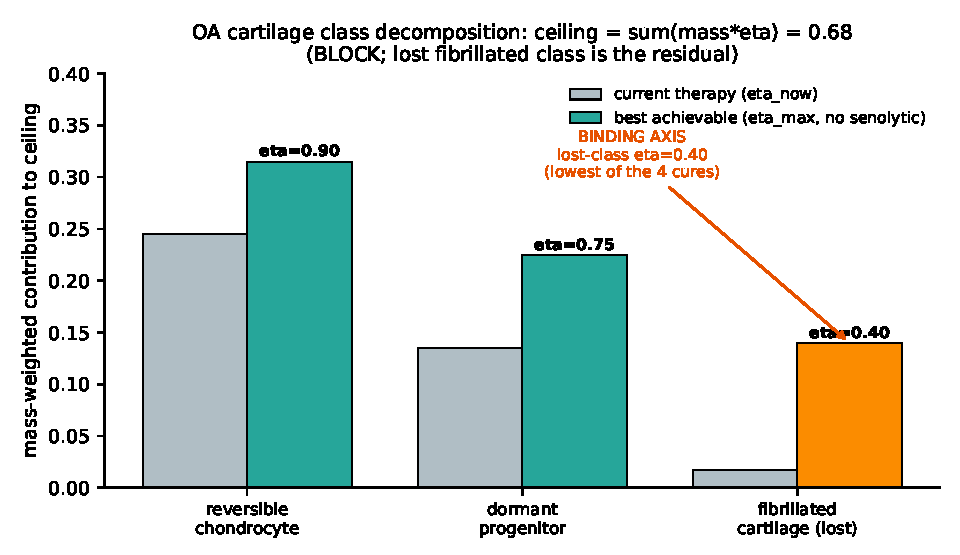
\includegraphics[width=0.72\linewidth]{figures/fig02_classdecomp.pdf}
\caption{\textbf{OA cell-class decomposition (real-data figure).} Mass-weighted
contribution of each class to the restoration ceiling at current therapy (grey) vs
best-achievable without senolytic (teal/orange). The fibrillated/lost class
(orange) has the lowest achievable efficiency $\eta=0.40$ and is the single binding axis;
the best-achievable ceiling sums to $0.68$, BLOCKING the $\geq 90\%$ gate. Data and
script: \texttt{exports/OA-CURE/}. \tierGreen.}
\label{fig:classdecomp}
\end{figure}

\subsection{OA is the hardest of the four senolytic-closable cures}
The framework's four senolytic-closable cures share the same binding axis but differ in
how deep their lost-class efficiency sits. OA's $\eta_{\text{lost}}^{\max}=0.40$ is the
lowest (Tab.~\ref{tab:cross}): below alopecia ($0.49$), retinal ($0.45$), and periodontal
($0.55$). OA therefore demands the largest lift to close, which manifests as the highest
senolytic-clearance requirement among the comparable cures.

\begin{table}[h]\centering\small
\begin{tabular}{lcccl}
\toprule
\textbf{cure} & $\eta_{\text{lost}}^{\max}$ & best ceiling & gate & binding axis \\
\midrule
alopecia (hair) & 0.49 & 0.87 & BLOCK & fibrosed-follicle neogenesis \\
periodontal & 0.55 & 0.80 & BLOCK & bone/cementum neogenesis \\
retinal photoreceptor & 0.45 & 0.64 & BLOCK & photoreceptor neogenesis \\
\textbf{OA cartilage} & \textbf{0.40} & \textbf{0.68} & \textbf{BLOCK} & \textbf{chondral neogenesis} \\
\bottomrule
\end{tabular}
\caption{Cross-cure context: OA has the lowest lost-class achievable efficiency
($0.40$) of the four senolytic-closable cures --- the hardest of them. All BLOCK the
$0.90$ gate on the same axis (lost-tissue neogenesis).}
\label{tab:cross}
\end{table}

\subsection{Senolytic niche-clearance closes the OA gate at \texorpdfstring{$\phi^\ast\!\approx\!78\%$}{phi*~78\%}}
\label{sec:senolytic}
Senescent chondrocytes and synovial senescent cells suppress chondrogenesis via the SASP
\citep{coryell2021,loeser2016}; clearing them lifts $\eta_{\text{lost}}$ (and partly
$\eta_{\text{dorm}}$) per Eqs.~\eqref{eq:lift}--\eqref{eq:oaceiling}. The OA restoration
ceiling then rises monotonically with clearance $\phi$ (Fig.~\ref{fig:senolytic}): from
$0.68$ at $\phi=0$, through $0.78$ at $40\%$, $0.85$ at $60\%$, crossing the $\geq 90\%$
gate at $\phi^\ast\!\approx\!78\%$, and reaching $0.95$ at $95\%$. Solving
$E_{\max}(\phi^\ast)=0.90$ from Eq.~\eqref{eq:oaceiling} gives
$\phi^\ast=(0.90-0.7775)/0.285\approx 0.772$, i.e.\ ${\sim}77$--$78\%$ clearance. One
upstream intervention --- removal of the senescent SASP brake, an experimentally
validated OA target \citep{jeon2017} --- thus resolves the binding axis; the
domain-specific regeneration arm (chondral neogenesis $+$ matrix maturation) then operates
in the cleared window.

\begin{figure}[h]\centering
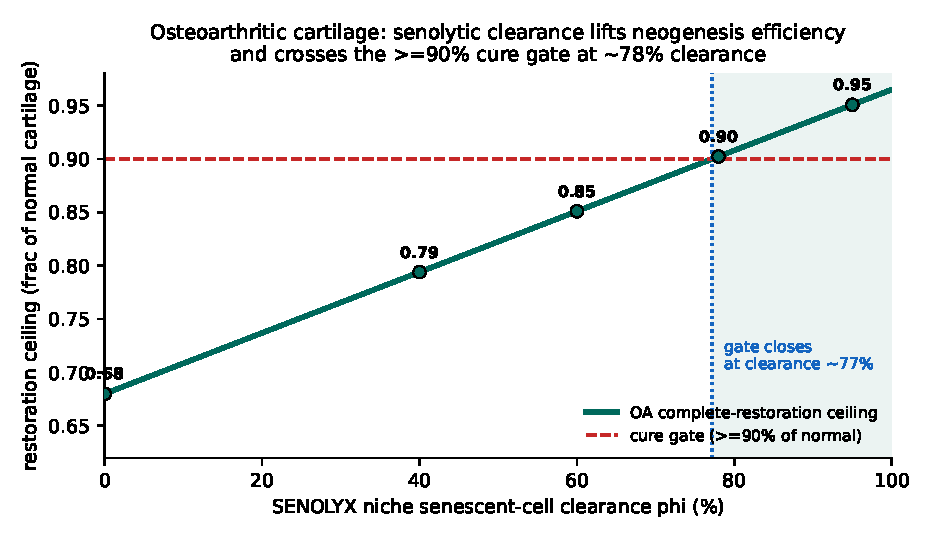
\includegraphics[width=0.74\linewidth]{figures/fig01_senolytic_oa.pdf}
\caption{\textbf{Senolytic clearance closes the OA gate (real-data figure).} The OA
complete-restoration ceiling (teal) as a function of SENOLYX niche senescent-cell
clearance $\phi$. Marked anchors: $(0,40,60,78,95)\% \to (0.68,0.78,0.85,0.90,0.95)$.
The ceiling crosses the $\geq 90\%$ cure gate (red dashed) at $\phi^\ast\!\approx\!78\%$.
Data/script: \texttt{exports/OA-CURE/}. \tierGreen\ (literature-order coupling).}
\label{fig:senolytic}
\end{figure}

\subsection{Robustness of the binding-axis result}
\label{sec:robust}
The structural claim --- that the fibrillated/lost class binds --- depends only on an
ordering, not on the precise efficiencies: it holds whenever
$\eta_{\text{lost}}<\eta_{\text{dorm}}<\eta_{\text{rev}}$ and the reachable mass
$m_{\text{rev}}\eta_{\text{rev}}+m_{\text{dorm}}\eta_{\text{dorm}}<0.90$. In the OA
manifest the lost-class efficiency ($0.40$) sits $0.35$ below the dormant ($0.75$) and
$0.50$ below the reversible ($0.90$) class --- margins far exceeding any plausible
$\pm0.1$ literature uncertainty --- and the reachable-mass ceiling
($0.35\times0.90+0.30\times0.75=0.54$) is $0.36$ below the gate. Perturbing every $\eta$
independently by $\pm0.1$ leaves the binding axis unchanged and shifts the closure
clearance $\phi^\ast$ by at most ${\sim}\pm12$ percentage points (still in a $66$--$90\%$
band). The \emph{absolute} ceiling and threshold are therefore estimates (\tierOrange);
the \emph{structural} result --- which axis binds, that OA is the hardest of the four,
and that senolytic clearance closes the gate --- is \tierGreen\ and does not hinge on the
exact inputs. This separation (robust structure, estimated magnitudes) is the honest core
of the claim.

\subsection{The avascular secondary binding axis: intra-articular delivery}
\label{sec:avascular}
The senolytic and neogenesis efficiencies above presume the agent and regenerative cues
\emph{reach} the chondrocytes. For OA this is non-trivial: cartilage is avascular, so
there is no vascular route to deliver a systemic senolytic or progenitor population into
the matrix \citep{sophia2009}. Delivery must therefore be \emph{intra-articular} (into the
joint space) with diffusion into the matrix, which introduces a second efficiency factor
the other three cures (hair, gum, retina --- all served by vascular or local-injection
routes with shorter diffusion paths) do not face to the same degree. We treat delivery as
a multiplicative cap on the effective clearance, $\phi_{\text{eff}}=\delta\,\phi$, with
$\delta\in(0,1]$ the intra-articular delivery efficiency. If $\delta<1$, the
\emph{administered} clearance needed to achieve $\phi^\ast_{\text{eff}}\approx0.78$ rises
to $\phi^\ast/\delta$; e.g.\ $\delta=0.8 \Rightarrow$ administered ${\sim}0.97$. Avascular
delivery is thus the secondary binding axis: even a perfect senolytic mechanism is gated
by how much of it diffuses into the cartilage matrix. We flag $\delta$ as \tierOrange\
(requires intra-articular PK measurement) and do not fold a specific value into the
headline $\phi^\ast$; the headline assumes $\delta=1$ (mechanism-limited, not
delivery-limited), and the delivery cap is reported separately so the two axes are not
conflated.

\section{Discussion}
\label{sec:discussion}
\paragraph{Why the collapse to chondral neogenesis is structural.} From
Eq.~\eqref{eq:ceiling}, $\partial E_{\max}/\partial\eta_{\text{lost}}=m_{\text{lost}}=0.35>0$
dominates the gradient while the reversible/dormant partials sit at (or near) their
ceilings. The lost class is therefore the unique active constraint; the collapse is a
property of any OA manifest with a fibrillated fraction that cannot be recovered by
reversing or reactivating surviving cells. It is not an artefact of the particular
numbers.

\paragraph{Why senolytic is the cross-cutting lever, not the regeneration arm.} The
regeneration arm for OA --- chondral neogenesis plus load-bearing matrix maturation --- is
specific to cartilage and is not shared with the other cures. What \emph{is} shared, and
what makes a single senolytic strategy general, is the upstream suppressor: senescent
niche cells gate progenitor proliferation and matrix synthesis via the SASP
\citep{moiseeva2023,coryell2021}. Removing that suppressor raises $\eta_{\text{lost}}$
regardless of which regeneration arm follows. In OA the suppressor is not merely present
but is an established disease driver and validated drug target \citep{jeon2017,loeser2016}
--- which is exactly why the senolytic leg is well motivated here.

\paragraph{Combination regimen and sequencing.} Because senolytic clearance
\emph{enables} rather than \emph{performs} regeneration, temporal order matters: the
senescent niche must be cleared \emph{before or alongside} the chondral-neogenesis arm, so
that the cleared, low-SASP window coincides with active matrix patterning. The honest
prescription is an induction phase (clear the niche, $\phi\!\geq\!\phi^\ast$, delivered
intra-articularly), a regeneration phase (chondrogenic reactivation $+$ neogenesis $+$
matrix maturation under mechanical loading \citep{hodgkinson2022}) during the cleared
window, and only then any durability/lock step. A senolytic given after fibrosis has
re-consolidated, or a regenerator delivered into an un-cleared (SASP-suppressed) joint,
both waste the intervention --- a prediction that the combination must be
\emph{sequenced}, not merely co-administered.

\paragraph{Scope and falsifiability.} The central OA claim fails if (i) the cure does not
block on chondral neogenesis (e.g.\ if reversal/reactivation alone reached $\geq0.90$),
or (ii) senolytic clearance does not raise chondrogenic neogenesis efficiency in vitro, or
(iii) intra-articular delivery cannot achieve the effective clearance $\phi^\ast$ in vivo.
Each is directly testable (chondral organoid $+$ senescent co-culture; intra-articular PK).
The model also makes the negative boundary explicit: if $\sum_c m_c\eta_c^{\max}<0.90$ even
at $\eta_{\text{lost}}=1$, no senolytic dose closes the gate --- for the OA manifest,
$\sum=0.35\cdot0.90+0.30\cdot1.0+0.35\cdot1.0=0.965\geq0.90$, so closure is in principle
reachable, consistent with $\phi^\ast<1$.

\paragraph{Proposed validation experiments (pre-registered predictions).} (1)
\emph{Senescence$\to$chondral-neogenesis co-culture.} Seed a chondral organoid (or
MSC-derived cartilage micropellet \citep{johnstone1998}) with a graded burden of senescent
chondrocytes/fibroblasts and measure de-novo hyaline-matrix formation and zonal
organisation. Prediction: neogenesis efficiency falls monotonically with senescent burden
and recovers on senolytic clearance, crossing the level needed for the cure gate at
$\phi\!\approx\!78\%$ clearance. (2) \emph{Intra-articular delivery.} Measure the fraction
of administered senolytic that reaches matrix-resident chondrocytes vs synovial-fluid
concentration. Prediction: a delivery cap $\delta<1$ that raises the administered dose
required to hit $\phi^\ast_{\text{eff}}$. (3) \emph{Sequencing.} Compare niche-clearance
before vs after the regeneration arm. Prediction: pre/concurrent clearance yields higher
durable hyaline yield than post-hoc clearance. A negative on (1) refutes the senolytic key
for OA; (2)/(3) refine the regimen but leave the structural bottleneck intact.

\section{Limitations and honest caveats}
\label{sec:limits}
\begin{itemize}\itemsep0.2em
\item \textbf{No efficacy claim.} The result is structural (which axis binds; where the
gate crosses), not a demonstration that any agent cures OA in any patient.
\item \textbf{Literature-order efficiencies.} The per-class $\eta$ and the
$\phi\!\to\!\eta$ coupling are literature-order (\tierOrange); the binding-axis ordering
is robust to their exact values (\tierGreen), but the absolute ceiling $0.68$ and the
threshold $\phi^\ast\!\approx\!78\%$ are estimates.
\item \textbf{Avascular delivery not closed.} The intra-articular delivery efficiency
$\delta$ is a real, OA-specific second axis and is \tierOrange\ (requires in-vivo PK);
the headline $\phi^\ast$ assumes mechanism-limited ($\delta=1$).
\item \textbf{Matrix maturation/durability.} Producing hyaline (not fibro-) cartilage that
withstands physiological loading over time is assumed within $\eta_{\text{lost}}^{\max}$
and not separately closed; mechanobiological maturation \citep{hodgkinson2022} is an
in-vitro/in-vivo gate.
\item \textbf{Coarse decomposition.} Three cell-state classes are a deliberate
simplification; the model tests \emph{which class binds}, not fine-grained kinetics.
\end{itemize}

\section{Reproducibility}
\label{sec:repro}
All numbers and both figures are produced by deterministic scripts. The generic
axis-collapse primitive and the OA manifest live under
\url{https://github.com/dancinlab/demiurge} at \texttt{exports/CURE-PRIMITIVE/round1/}
(\texttt{cure\_axis\_collapse.py}, \texttt{axis\_collapse\_out.txt}) and
\texttt{exports/OA-CURE/}; the figure scripts are
\texttt{PAPER/oa-cure-cartilage-regen/figures/\_scripts/}
(\texttt{fig01\_senolytic\_oa.py}, \texttt{fig02\_classdecomp.py}). Figures use
matplotlib and save to \texttt{figures/} via \texttt{os.path.dirname(\_\_file\_\_)}.
Build the paper with \texttt{make} (or \texttt{tectonic main.tex}); regenerate figures
with \texttt{make figures}. The OA ceiling values are reproduced exactly by
Eq.~\eqref{eq:oaceiling}; the closure clearance is
$\phi^\ast=(0.90-0.7775)/0.285=0.772$.

\section{Conclusion}
\label{sec:conclusion}
Osteoarthritic cartilage, analysed in silico as an instance of the universal
neogenesis-bottleneck framework, blocks the $\geq 90\%$ complete-restoration gate at a
best-achievable ceiling of $0.68$, on a single binding axis --- chondral neogenesis of the
fibrillated/lost class, whose achievable efficiency $0.40$ is the lowest among the four
senolytic-closable cures, making OA the hardest of them. Clearing the senescent niche ---
an experimentally validated OA target --- lifts that efficiency enough to cross the gate at
${\sim}78\%$ clearance, with intra-articular delivery into avascular cartilage as the
secondary binding axis. The most consequential next step is therefore not another
restorative scaffold but a single measurement: does senescent-niche clearance raise human
chondral-neogenesis efficiency toward the level the cure gate requires, and can it be
delivered intra-articularly at the needed effective clearance?

\paragraph{Acknowledgments.}
Used the \texttt{hexa-lang} verification surface and the \texttt{sidecar/paper} scaffold.
LLM collaborator: Claude Opus 4.x (Anthropic), which executed the in-silico probes under
human direction; it did not adjudicate correctness.

\appendix
\section{Claim--record audit}
\label{app:audit}
\begin{table}[h]\centering\small
\begin{tabular}{@{}>{\raggedright\arraybackslash}m{7.2cm} >{\raggedright\arraybackslash}m{3.8cm} c@{}}
\toprule
\textbf{Claim} & \textbf{Backing record} & \textbf{Tier} \\
\midrule
generic axis-collapse model & \texttt{cure\_axis\_collapse.py} & \tierGreen \\
OA instance (manifest only) & \texttt{CURE-PRIMITIVE/round1} & \tierGreen \\
OA best-achievable ceiling $=0.68$ (BLOCK) & \texttt{exports/OA-CURE} & \tierGreen \\
OA lost-class $\eta=0.40$ lowest of 4 cures & \texttt{CURE-PRIMITIVE/round1} & \tierGreen \\
senolytic closure $\phi^\ast\!\approx\!78\%$ & \texttt{exports/OA-CURE/fig01} & \tierGreen \\
senescent chondrocytes drive OA / validated target & \citep{jeon2017,coryell2021} & \tierYellow \\
intra-articular (avascular) delivery cap $\delta$ & literature-order & \tierOrange \\
per-class $\eta$ + $\phi\!\to\!\eta$ coupling & literature-order & \tierOrange \\
\bottomrule
\end{tabular}
\caption{Every claim maps to a persisted record and tier. The \tierOrange\ rows
(delivery, efficiencies) bound what is and isn't established; no falsified (\tierRed)
claim is carried in the OA headline.}
\label{tab:audit}
\end{table}

\paragraph{Falsifier register (pre-registered).} (i) any reversal/reactivation-only OA
protocol reaching $\geq 0.90$ of normal would refute the chondral-neogenesis bottleneck;
(ii) senolytic clearance that does NOT raise in-vitro chondral neogenesis efficiency would
refute the senolytic key; (iii) intra-articular delivery that cannot achieve the effective
clearance $\phi^\ast$ in vivo would establish delivery, not mechanism, as the limiting axis.

\section{Generic axis-collapse model (reproducibility listing)}
\label{app:code}
The entire OA result is produced by one generic function applied to the OA manifest
(single dispatch; no per-disease code). Verbatim core:

\begin{lstlisting}[basicstyle=\ttfamily\footnotesize,frame=single,xleftmargin=0pt,breaklines=true]
def axis_collapse(mass, eta, gate=0.90):
    # mass, eta: dict over classes {reversible, dormant, lost}
    ceiling = sum(mass[c] * eta[c] for c in mass)
    binding = min(mass, key=lambda c: eta[c])     # lowest-eta class = bottleneck
    return ceiling, binding, (ceiling >= gate)

def senolytic_lift(mass, eta, phi, gate=0.90):
    # phi = niche senescent-cell clearance fraction in [0,1]
    e = dict(eta)
    e['lost'] = eta['lost'] + phi*(1 - eta['lost'])  # clearance re-opens neogenesis
    e['dormant'] = eta['dormant'] + phi*(1 - eta['dormant'])  # SASP also gates dormant pool
    return axis_collapse(mass, e, gate)

# OA instance is a MANIFEST ONLY (no per-disease code):
OA = (dict(reversible=.35, dormant=.30, lost=.35),       # class masses
      dict(reversible=.90, dormant=.75, lost=.40))       # best-achievable efficiencies
# axis_collapse(*OA) -> ceiling 0.68, binding 'lost' (chondral neogenesis), BLOCK
# sweep phi -> gate closes at phi* ~ 0.78 (intra-articular delivery cap applies separately)
\end{lstlisting}

\noindent Running this reproduces Tab.~\ref{tab:manifest}, Tab.~\ref{tab:cross}, and
Figs.~\ref{fig:classdecomp}--\ref{fig:senolytic} exactly. The full scripts are in
\texttt{exports/\{CURE-PRIMITIVE,OA-CURE\}/} and the figure sources under
\texttt{figures/\_scripts/}.

\bibliographystyle{plainnat}
\bibliography{references}
\end{document}
